% ----------------------------------------------------------
% Consciousness subsection
% ----------------------------------------------------------
\subsection{Consciousness}
A logical moment can be formed by a division (first moment) or by logical subdivisions (other moments).
	\begin{figure}[H]
	\caption{Logical interval}
	\label{fig:consciousness_logical_moments}
	\centering
	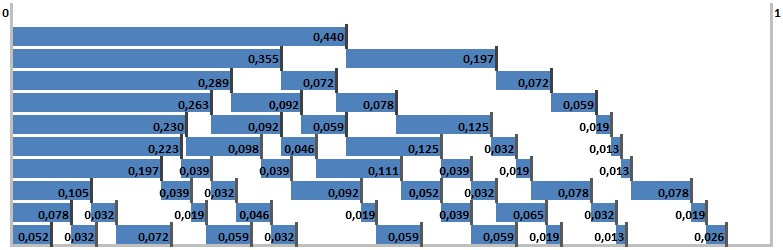
\includegraphics[scale=.7]{sections/images/consciousness_logical_moments.jpg}
	\floatfoot{Example of a logical interval with ten logical moments.}%\footnotemark}
	\end{figure}
	%\footnotetext{Fonte: note}

The units of logical moments tend to form the largest and most complex logic in the population, the largest wave, consciousness.
	\begin{figure}[H]
	\caption{Conscious logical interval}
	\label{fig:consciousness}
	\centering
	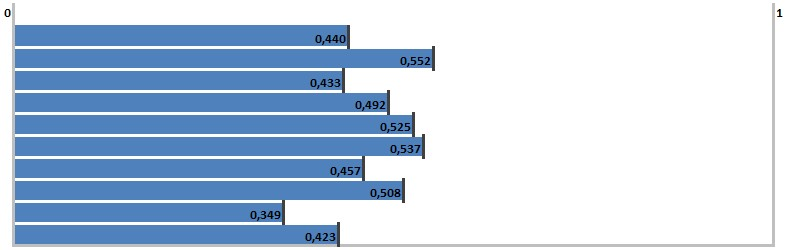
\includegraphics[scale=.7]{sections/images/consciousness.jpg}
	\floatfoot{Example of a conscious logical interval with ten units of logical moments.}%\footnotemark}
	\end{figure}
	%\footnotetext{Fonte: note}

It can be seen in Table \ref{tab:10000_all} that the probability of 99.99\% of the samples in a population (Range), which increase in quantity as the logical moments increase, tends to be increasingly in the center of the logical interval and this centralization tends to infinity.
	\begin{figure}[H]
	\caption{Centralization of 99.99\% of the samples}
	\label{fig:centering_of_99_range}
	\centering
	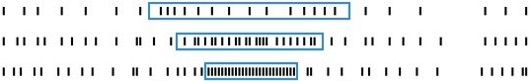
\includegraphics[scale=1]{sections/images/centering_of_99_range.jpg}
	\floatfoot{Tendency to center the range of 99.99\% of the samples.}%\footnotemark}
	\end{figure}
	%\footnotetext{Fonte: note}

The largest wave of a population tends to a histogram of the normal distribution, as shown in Figure \ref{fig:trend_chart_of_normal_distribution}. All aspects listed below are inherent in the logical abstraction called consciousness, they are emergent logics of primordial logic.

The first sample of a population already a discrepancy (an interval), therefore it already applies all the characteristics of the conscience, the biggest discrepancy of the population. In this way, there is no possibility of a population expansion that does not have at least one discrepancy. This discrepancy or interval will be rising to the left, centralized, to the right or simultaneously in any of these possibilities, according to the movement described in the Space subsection.

\subsubsection{Infinite}
One of the most important aspects that the negation of nothingness brings (negation of self), is infinity, that is, in any logical interval the infinite fits again. The primordial logic that started the entire logical interval is the same found in its subsequent intervals (subintervals). This substantiates how a high-level logic like the human subconscious explains primordial logic, since it is not necessary to go back to the first logical moment of the interval to deduce it, as this phenomenon is omnipresent throughout the interval. This phenomenon can be seen in the subsection on Space, Spatial plane.

\subsubsection{Waves}
Probabilistically, the distribution of new samples from a population tends to concentrate more samples toward the median of the population as the frequency of samples increases in this direction. However, the distribution of these samples with uniform growth frequencies is infinitesimal compared to the random possibilities of this growth. Thus, the tendency of these growth frequencies toward the median, together with the very low (infinitesimal) probability of this growth being uniform, leads to frequencies in the waveform. The relationship of the density or amplitude of a wave to its length is detailed in the next subsection.
	\begin{figure}[H]
	\caption{Waveform}
	\label{fig:consciousness_waves}
	\centering
	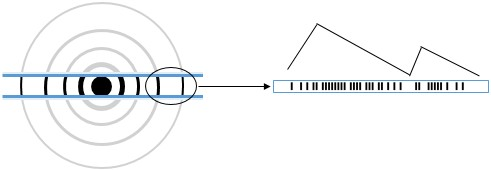
\includegraphics[scale=.8]{sections/images/consciousness_waves.jpg}
	\floatfoot{Wave pattern inferred by the trend of this distribution with higher frequencies towards the population median and very low probability of uniform growth of these frequencies.}%\footnotemark}
	\end{figure}
	%\footnotetext{Fonte: note}

Merging one wave into another eliminates its discrepancy and makes that wave cease to exist and become part of the first wave, which has its peak closer to the median, in this example. A wave doesn't die, it just merges with another wave closer to it.
	\begin{figure}[H]
	\caption{Wave unification}
	\label{fig:consciousness_uniform_wave}
	\centering
	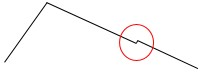
\includegraphics[scale=1]{sections/images/consciousness_uniform_wave.jpg}
	\floatfoot{Waves being unified to exemplify the uniform growth of the samples.}%\footnotemark}
	\end{figure}
	%\footnotetext{Fonte: note}

\subsubsubsection{Wavelength and amplitude}
The histogram is used in the figures in this subsection and later to facilitate visualization and understanding of the distribution of samples in a population, because it represents very well the density curves of a population, according to the different views of the Figure \ref{fig:consciousness_wave_histogram}, representing only one interval or wavelength paired by the median of the population.  
	\begin{figure}[H]
	\caption{Histogram in different views}
	\label{fig:consciousness_wave_histogram}
	\centering
	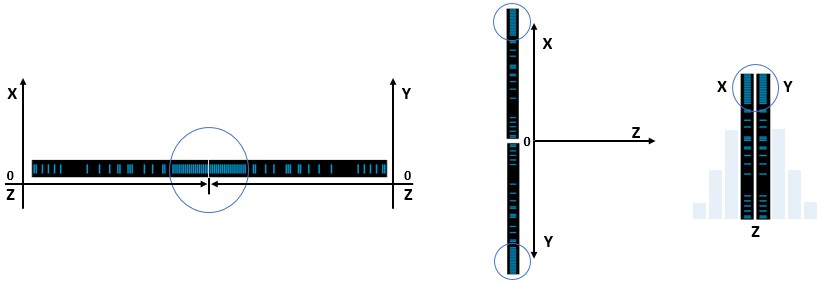
\includegraphics[scale=.7]{sections/images/consciousness_wave_histogram.jpg}
	\floatfoot{Different ways of population representation in a histogram.}%\footnotemark}
	\end{figure}
	%\footnotetext{Fonte: note}}

The real or natural numbers, described in the subsection of the Central limit theorem, are just mathematical devices to facilitate understanding and are not present at this logical level. Therefore, an interval has its base on the side with the lowest density of samples and its direction goes from the base to the side with the highest density of samples, like the representation of the Z dimension in Figure \ref{fig:consciousness_wave_histogram}. If a region of the population is in perfect balance in its distribution, it is not a discrepancy, therefore it is not an interval and this concept of base and direction does not apply.
	
The length and amplitude of waves establish a quantity-per-interval or unit relationship. These units are established by wave entanglement, as seen in the next subsection. Thus, amplitude is the density of a wavelength, the density of some interval.  

When adding a new sample to the population, the entire interval is proportionally distributed to match that sample, as shown in Figure \ref{fig:consciousness_space_volume_amplitude}.
	\begin{figure}[H]
	\caption{Interval expansion}
	\label{fig:consciousness_space_volume_amplitude}
	\centering
	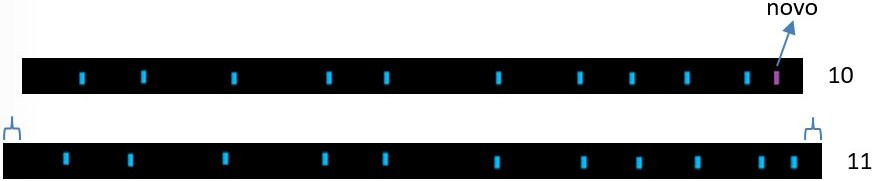
\includegraphics[scale=.5]{sections/images/consciousness_space_volume_amplitude.jpg}
	\floatfoot{Expanding the interval by adding new samples.}%\footnotemark}
	\end{figure}
	%\footnotetext{Fonte: note}}
	
In large intervals with many logical moments, a smaller proportional discrepancy of wave amplitudes is observed. This characteristic is related to the larger number of logical moments and possible subintervals that can more easily compensate and neutralize the probabilistic unevenness of the interval. The larger the intervals, the more balanced they grow towards the population median (probabilistically) as seen in Figure \ref{fig:consciousness_space_subconsciousness}. More complex intervals with this feature can represent, for example, the universe, then galaxies, stars, planets, etc.
	\begin{figure}[H]
	\caption{Wave amplitude at large intervals or lengths}
	\label{fig:consciousness_space_subconsciousness}
	\centering
	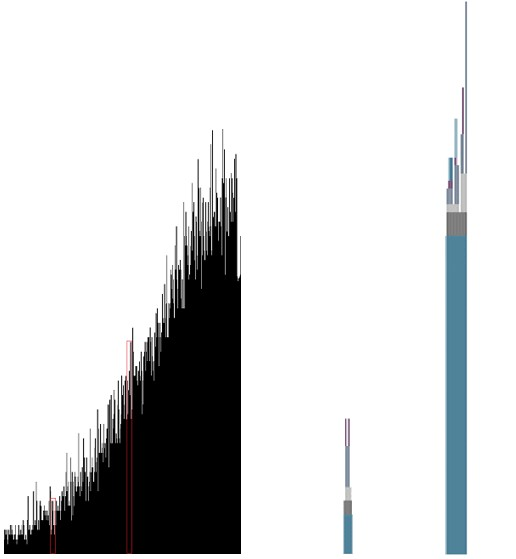
\includegraphics[scale=.45]{sections/images/consciousness_space_subconsciousness.jpg}
	\floatfoot{Smaller wave discrepancy at large intervals.}%\footnotemark}
	\end{figure}
	%\footnotetext{Fonte: note}

At smaller intervals and with many logical moments, a greater proportional discrepancy of wave amplitudes is observed. In these intervals smaller object systems can be observed. The smaller the intervals are, the more unbalanced they will grow towards the population median (probabilistically) as seen in the figure \ref{fig:consciousness_space_subconsciousness_min}. More complex wave systems with this feature can represent, for example, the atom, which is very small, present in huge quantities, and the particles orbiting its nucleus (electrons) are much more distant from it. This greater discrepancy is strictly linked to the reduced size of these intervals, making them receive these new samples in a less uniform and unbalanced way, which makes the follow-up of their subintervals to their peak or to their reference line less accurate (the spiral becomes wider, elongated and misshapen due to less uniformity in its correction frequency). Spiral and orbits can be seen in more detail in the subsection on Spiral and orbit.
	\begin{figure}[H]
	\caption{Wave amplitude at small intervals or lengths}
	\label{fig:consciousness_space_subconsciousness_min}
	\centering
	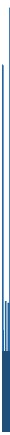
\includegraphics[scale=.45]{sections/images/consciousness_space_subconsciousness_min.jpg}
	\floatfoot{High wave discrepancy at small intervals.}%\footnotemark}
	\end{figure}
	%\footnotetext{Fonte: note}}

\subsubsubsection{Entanglement}
The most similar samples in terms of frequency and distribution are the samples that are part of the same wave. They are non-overlapping, opposite frequencies that complete each other.

Probabilistically, the two complementary parts of a wave tend to be at approximately equal distances, equidistant from the median, but this is not a rule and the complementary parts of a wave may be at different distances from the median. The phenomenon of parity of the parts of a wave is called wave entanglement.

These pairs are formed by the probability distribution of the population and are part of the same probabilistic unit.

These probabilistic units form smaller waves (subconsciousnesses), similar to the largest wave in the entire interval, usually entangled by the population median (consciousness). Consciousness is the logic of the entire interval, while it forms subconsciousnesses or sublogics, like small waves of a larger wave. These small waves are similar to the pattern of the larger wave.
	\begin{figure}[H]
	\caption{Subconsciousness}
	\label{fig:consciousness_subconscious}
	\centering
	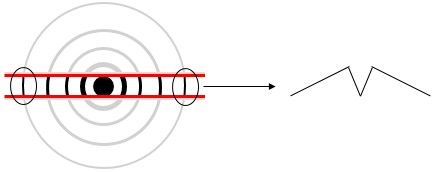
\includegraphics[scale=.8]{sections/images/consciousness_subconscious.jpg}
	\floatfoot{The wave pattern forms subconsciousnesses similar to the pattern created by consciousness, as seen in Figure \ref{fig:trend_chart_of_normal_distribution}.}%\footnotemark}
	\end{figure}
	%\footnotetext{Fonte: note}
	
The entanglement of waves can occur at different levels or intervals, as seen in Figure \ref{fig:consciousness_subconscious_entanglement}, which forms nested wave systems. The borderless braces (right) identify the intervals at which a new sample triggered the jump, as seen in the next subsection. The numbered arcs indicate the order of the entanglements. An entanglement can occur equidistantly from the median without the jump, like the first entanglement (violet).

The largest entanglement is shown in the examples in Figure \ref{fig:consciousness_subconscious_entanglement} as the first entanglement (violet), which occurred when that interval was the smallest, probably.  Large intervals tend to be kept ordered by the reordering of their subintervals subsequently. The largest wave is commonly entangled by the population median.
	\begin{figure}[H]
	\caption{Wave entanglement levels - wavelengths}
	\label{fig:consciousness_subconscious_entanglement}
	\centering
	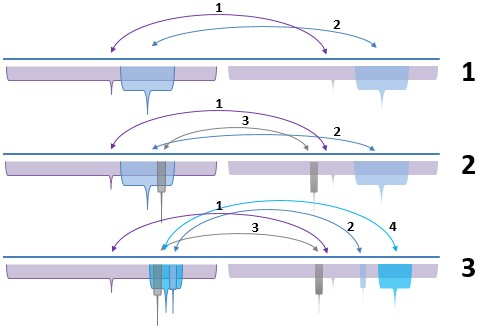
\includegraphics[scale=.8]{sections/images/consciousness_subconscious_entanglement.jpg}
	\floatfoot{Examples of entanglement levels of waves or levels of wavelengths.}%\footnotemark}
	\end{figure}
	%\footnotetext{Fonte: note}

If several intervals are part of the same population discrepancy, of the same wave, then these are subintervals of a larger interval, of a larger wave.

The possible wavelengths of a population are defined by these levels of wave entanglement. Thus, regardless of the order of the jumps, larger entanglements are the longer wavelengths and smaller entanglements are the shorter wavelengths, which allows larger waves to have smaller subwaves. 

A superior interval can change its entangled pair (the remaining samples that are not part of its subintervals) without affecting its subintervals, that is, each interval or subinterval has its best matching pair independently. This is an extraordinary condition because of the similarity conditions required for entanglement.

Larger waves are formed by adding their new samples, and can form new subintervals. The meeting or separation of two entanglements does not entail a new entanglement. Thus, larger waves are also formed through the inclusion (vigor of entanglement) of smaller waves already entangled when the areas of these waves are partially or totally overlapping.

NOTHING \underline{NOT BEING} is synonymous with movement, with change, as presented in the opening section of this article, Logic. In this way, movement is the signature of an interval. This signature corresponds to the distribution of samples within the interval, as per the Space subsection. Intervals with similar signatures tend to have similar motions and speeds, tend to be at the same discrepancy as a larger wave. This characteristic differentiates one interval from another, in other words, it discriminates discrepancies in a population.

Virtual intervals are non-entangled intervals, which usually form virtual clouds. These virtual clouds are sets of virtual intervals that exchange their entangled pairs constantly. These virtual intervals move according to the spatial dimensions of their side of the pair, best visualized in the Space subsection. An interval that has lost its entanglement, resulting in a virtual interval, will continue its trajectory until it entangles again, eventually with a jump. Virtual intervals can grow and stabilize to become a non-virtual interval.

The vigor of an entanglement is the number of subintervals that one wave has entangled with another. Vigor is total when a subinterval (which is also a wave) has entangled all its subintervals within its superior wave, that is, all its subintervals are fractions of its superior interval. Total vigor occurs more easily when the waves of a system are born with the system, so the greater the interval, the greater the number of possible subintervals and the greater the chances of them becoming entangled with each other, due to the probabilistic distribution of the population (the samples are predisposed yet random), which makes these intervals more and more stable as they grow. It is also possible to have total vigor when one interval converges with another and remain that way for a period in which its subintervals are influenced by the peak of the system, to the point that their entangled pairs are within the same population discrepancy even though they were not born of this population discrepancy to which they came to belong. The amount of subintervals that a wave is constantly sharing with another wave is what guarantees a greater or lesser synchronism of the movements of these waves, according to the subsection of Space. This sharing can occur with already entangled subintervals or with unentangled subintervals, usually part of a virtual cloud. This sharing can also occur on only one side of the entangled pair, as in the case of waves of the same level.

As an example of partial vigor, the entanglement of waves or larger parts of a car (car parts) can occur with greater to lesser vigor, such as the fusion of parts or welding, glues, something more elastic, among others. Thus, the engine and wheels of a car when accelerating and braking respectively, equally accelerate and decelerate its entangled parts. The less vigorous the entanglements, the more the parts suffer from inertia, such as loose objects and occupants inside a vehicle. Another example of the partial vigor of entanglement can be seen in molecular bonding.

As an example of total vigor are galactic, stellar, and nuclear systems, the latter being less stable due to its small size. However, all these systems have a high level of synchronism in their motions, better explained in the Space subsection.

\subsubsubsection{Jump}
In Figure \ref{fig:consciousness_space_subconscious_observation_jump} a new entanglement of already entangled intervals is observed (represented by columns of a histogram to facilitate the visualization of the interval). This new entanglement occurs as the samples of the entangled pairs are no longer equivalent with the addition of new samples on one side of the pair.
	\begin{figure}[H]
	\caption{New entanglement}
	\label{fig:consciousness_space_subconscious_observation_jump}
	\centering
	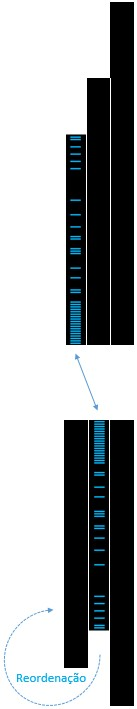
\includegraphics[scale=.53]{sections/images/consciousness_space_subconscious_observation_jump.jpg}
	\floatfoot{New entanglement caused by the non-equivalence of the entangled pair with the addition of new samples on one of its sides.}%\footnotemark}
	\end{figure}
	%\footnotetext{Fonte: note}

Jumping occurs when an interval entangles with a virtual interval (non-entangled interval). In this case, the entangled interval appeared in one region and when entangled again with another virtual interval, it appeared in another.

As an example, a photon entering the electron's interval can unbalance one side of the electron's entangled pair, which makes it jump, but since the electron's interval is small and the photon is fast (because it is even smaller) it quickly leaves the electron's interval, which becomes unbalanced again and returns to the energy level equivalent to the one before the jump.

\subsubsection{Time}
Time only makes sense when observed in a specific population expansion (partially), when observed in its entirety it is a transcendent constant that mirrors a probabilistic matrix of infinite possibilities.

\subsubsubsection{Integral}
In the initial section Logic (the genitor section of all the others in this article) it was presented that logic is a sequence of negations of itself at time zero, that is, at no point between its negations does logic go to \underline{BEING}, guaranteeing the primordial premise of the logic constant, \underline{NOT BEING}. When the expansion is generalized each logical moment is in infinitely different orders within the infinite population expansions of this constant, that is, the primordial logical \underline{NOT BEING} is similar to a probabilistic n x n matrix when generalized, it is a transcendent constant that mirrors or represents these infinite possibilities. In this way, the order of each logical moment only makes sense in the expansion of a specific population. In the observer-driven experience of time, the ordering of each sequence is the essence of this logical quantity and therefore more relevant than its origin, which is of a simultaneous nature, transcending time.

\subsubsubsection{Partial}
Time is the addition of new logical moments between existing moments as the self-negation of primordial logic proceeds. The changes are cumulative and as the number of logical moments increases, the less relevant each new moment within the conscious interval will be. One in a hundred is more relevant than one in a thousand. 
	\begin{figure}[H]
	\caption{Time}
	\label{fig:consciousness_time}
	\centering
	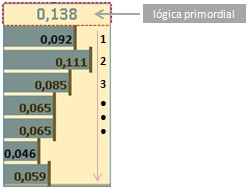
\includegraphics[scale=.8]{sections/images/consciousness_time.jpg}
	\floatfoot{Progression of time as logical moments advance.}%\footnotemark}
	\end{figure}
	%\footnotetext{Fonte: note}

Time also passes in intervals when they converge with other intervals and are able to interact by colliding or entangling their sub-intervals, according to the next subsection of Space.

Each population has a different order in its sequence and it is this order that gives rise to the logical quantity called time. It is this order of the universe or of consciousness that will give the notion of what happens before or after, that is, the past, the present and the probabilistic future prospections.

Temporal flows of a population can have the same beginning and even the same temporal expansion, infinitely, from the first negation of the expansion. Thus, there are infinite temporal flows in the same population expansion at different points in it, as the highlighted expansion in Figure \ref{fig:consciousness_constant_time}. Therefore, it makes no sense to associate the number of samples or the age of the temporal flow of a particular universe with the age of the logical constant \underline{NOT BEING}, which precedes time. Motion, change or time are smaller versions of what is constant and total.
	\begin{figure}[H]
	\caption{Logical constant - population time flows}
	\label{fig:consciousness_constant_time}
	\centering
	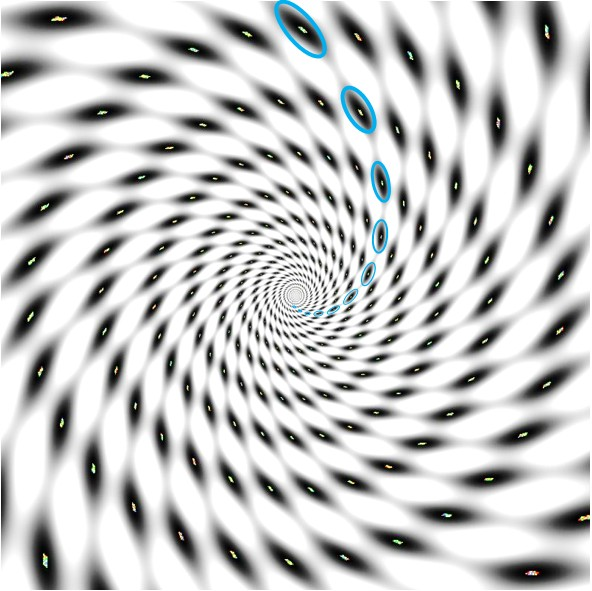
\includegraphics[scale=.6]{sections/images/consciousness_constant_time.jpg}
	\floatfoot{Source: Twitter, 2022. \protect\footnotemark}
	\end{figure}
	\footnotetext{\url{https://twitter.com/akiyoshikitaoka/status/851375952051421184}}

Another important factor when observing time (the observer is more detailed in the consciousness subsection – Observer and life) is that, probabilistically, subconsciousnesses or intervals closer to the population median will have a larger addition of new samples in their intervals, which are directly observed by these subconsciousnesses. On the other hand, subconsciousnesses far from the population median will have a smaller addition of samples in their intervals and are subject to a larger number of indirectly induced changes, as detailed in the next subsection of Space and that can also be seen in Figure \ref{fig:consciousness_space_volume_amplitude}.  This phenomenon of temporal observation provided by the probability of the population distribution avoids the twin paradox \cite{twin_paradox}.

When the gravitational attraction is stronger the samples are more intensely distributed in this gravitational direction, which to some extent opposes a looser movement in other directions or orbits. This characteristic may influence the movement of atomic clocks, which may have a more uniform movement in environments with low gravity.

Prospections of the observer's future are based on the probabilistic distribution of the population and, therefore, on the probabilistic distribution of each sub-interval of the population. The universe tends to be probabilistic, while random at levels of detail (which makes events different), yet predictable at some level, as shown in Figures \ref{fig:consciousness_logical_moments} and \ref{fig:consciousness}. 

\subsubsection{Space}
Time and space come from the same population samples. Time is related to the order of each sample, while space deals with their disposition in the population at each new order.

\subsubsubsection{Spatial plane}
The spatial plane is the representation of the infinite, of the \underline{NOT BEING} in all its possibilities and from which the space-time flows emerge as its possibilities. That is, it is the representation of NOTHING, the void that mirrors or represents all possibilities and it is present at all scales between any spatial and temporal possibility. This plane also emerges within the scales of thought, where the exercises of prospections (future possibilities) emerge from the probabilities of a determined interval with this plane or logical flow of infinite possibilities. So, when thinking about NOTHING naturally this logical representation of empty and infinite space emerges.

The spatial plane is logical and flat even though your samples tend, probabilistically, towards the reference line of the largest wave, which tends to be separated by the population median.
	\begin{figure}[H]
	\caption{Flat universe}
	\label{fig:consciousness_flat_universe}
	\centering
	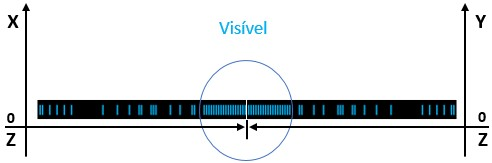
\includegraphics[scale=.6]{sections/images/consciousness_flat_universe.jpg}
	\floatfoot{Concentration of 99\% of samples.}%\footnotemark}
	\end{figure}
	%\footnotetext{Fonte: note}

\subsubsubsection{Dimensions}
NOTHING \underline{NOT BEING} is synonymous with movement, with change, as presented in the opening section of this article, Logic. In this way, as shown in Figure \ref{fig:consciousness_flat_universe}, the Z is the representation of the number of samples of a wave. Therefore, Z is the representation of entanglements, which is the only authentic and genuine dimension (the essence of spatial dimensions), being the main direction of movement. As the amount of samples only increases (the same reason that makes time only flow in one direction), the intervals will also move in that predominant direction, which in this case is up. The X and Y are just subdimensions that represent the density, the peak, on each side of the entangled pair respectively, that is, they manifest the different ways that Z rises (quantity), and X and Y (density) can be anywhere (left, right, centered, etc.) within each side of the entangled pair. These movements are more detailed in Figure \ref{fig:consciousness_space_plan_nosubinterval}. Later the X, Y and Z will be treated as dimensions to facilitate understanding.

It is easier to understand the entanglement when looking at Figure \ref{fig:consciousness_space_dimensions}. In part (A) of the Figure, it is shown how each side of the pair behaves in their respective dimensions and subdimensions, in parallel. It is easy to see that intervals with similar movements will meet and the parts of these intervals and subintervals that correspond on each side of the pair become entangled, like the overlapping area of the ellipse in part (B).
	\begin{figure}[H]
	\caption{The movements of the pairs and the encounter - entanglement}
	\label{fig:consciousness_space_dimensions}
	\centering
	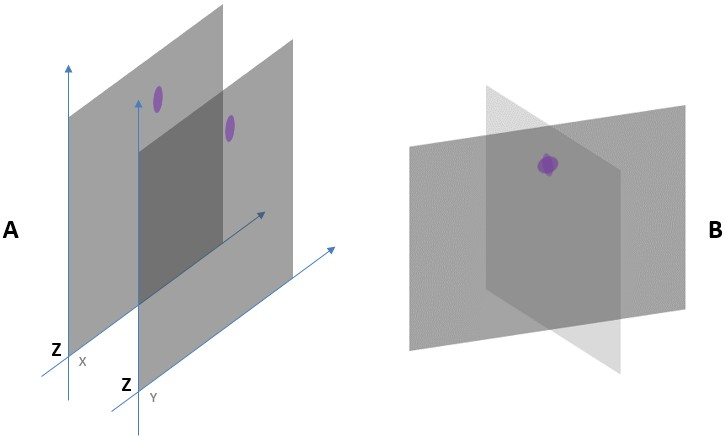
\includegraphics[scale=.7]{sections/images/consciousness_space_dimensions.jpg}
	\floatfoot{Movements in the respective dimensions and subdimensions of each side of the pair underlies the entanglement.}%\footnotemark}
	\end{figure}
	%\footnotetext{Fonte: note}

When a human being moves, goes from one point to another and returns (zigzag), or any other movement, he is making a movement similar to a spiral. Observing the movement as a whole, the human being is also moving through the planet, solar system, galaxy, etc. No matter what dimensions the movement used, probabilistically, the movements tend to be smooth, no matter how abrupt they seem locally (left or right, up or down, front or back). Movements tend to be a variation of the Spiral, as per the subsection on Spiral and orbit.

\subsubsubsection{Movement}
Each new sample is time and also space (motion and change). Movement is a signature of an interval and that signature corresponds with the distribution of samples within the interval. A subinterval, which does not contain a subinterval as in Figure \ref{fig:consciousness_space_plan_nosubinterval}, can be born anywhere. These virtual intervals move according to the spatial dimensions of their side of the pair when not entangled and with the dimensions of both sides of the pair when entangled. In Figure \ref{fig:consciousness_space_plan_nosubinterval}, an interval is shown that does not yet contain subintervals, so its rise will either be centralized if its samples are evenly distributed or with a centralized peak, or it will be skewed to the right or left as the higher concentration of samples is on one side (it is more common for the concentration of samples to be towards the median of the population). In the virtual interval the dimensions are Z (to go up) and X or Y, depending on the side of the pair, for the sample density of the non-entangled interval. In the tangled interval the analogy is the same as in the virtual interval, but the dimensions are Z (to go up on both sides of the pair), X and Y for the sample density of the interval on each side of the tangled pair. A non-rarefied environment can hinder these movements because of collisions.
	\begin{figure}[H]
	\caption{ Interval without subintervals}
	\label{fig:consciousness_space_plan_nosubinterval}
	\centering
	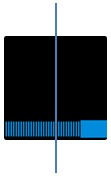
\includegraphics[scale=.7]{sections/images/consciousness_space_plan_nosubinterval.jpg}
	\floatfoot{ Moving an interval without subintervals.}%\footnotemark}
	\end{figure}
	%\footnotetext{Fonte: note}

Theoretically, the maximum speed is 1 unit of space per 1 unit of time, that is, intervals move at a speed lower than 1 unit of space per 1 unit of time. It's not because you have more samples that you have more speed. If an interval has 2 samples to the right, for example, it will move approximately 2 space units per 1 time unit, that is, approximately 1 space unit for each sample. Thus, an interval has a speed limit of 1 space unit per sample per 1 time unit. The fastest interval, hypothetically, would be the interval with a single sample totally centralized or totally to the right or left of the interval, so this interval would reach the maximum speed, but there will always be an even more centralized sample, to the right or left of an infinite interval, according to the interval characteristics shown in Figure \ref{fig:primordial_logic_representation}.

The speed of an interval is not directly related to the number of samples, but to the proportion of distribution of these samples. The more disproportionately distributed an interval is, the more concentrated its peak can be, the faster the interval will be, regardless of direction. Therefore, both smaller and larger intervals can have high velocities, and extremely large intervals have greater ease in concentrating the peak, increasing its disproportion.

A subinterval that is born within its upper interval is born fully synchronized with this upper interval, that is, the samples of the subintervals are also samples of the upper interval, they are shared samples, according to the vigor of their entanglements, as seen in the subsection of Entanglement. In Figure \ref{fig:consciousness_space_plan}, the sum of the motions of the subintervals of a higher interval moves that interval with a given direction and speed, which also carries with it those smaller subintervals that are part of it, even though these subintervals may diverge and leave the higher interval at a given moment. In this way, the movements of the smaller waves were the movement of the largest wave of the population, where its direction and speed are predominantly of the majority, usually the peak, notwithstanding the movement of the minorities. And like a block, the movement of the largest wave leads to the smaller ones, which are parts of it, even though some of these smaller waves have their own movement and can escape at a given moment by divergence in their directions from the direction of the majority.
	\begin{figure}[H]
	\caption{Spatial distribution and movement}
	\label{fig:consciousness_space_plan}
	\centering
	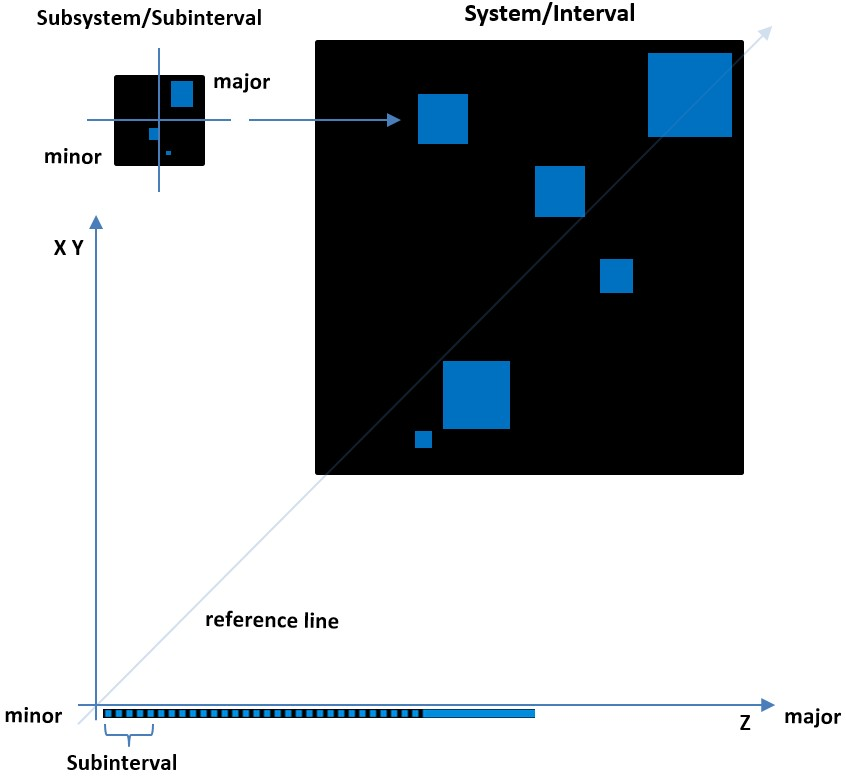
\includegraphics[scale=.6]{sections/images/consciousness_space_plan.jpg}
	\floatfoot{Spatial distribution and movement of subintervals and population interval.}%\footnotemark}
	\end{figure}
	%\footnotetext{Fonte: note}

Intervals that have subintervals can move in any direction, since their intervals that don't have subintervals, as in Figure \ref{fig:consciousness_space_plan_nosubinterval}, can tangle anywhere and thus this interval can have a distribution of subintervals in any direction, according to Figure \ref{fig:consciousness_space_plan}. The situation in which an interval goes down (Z dimension) is very rare, even rarer when the interval grows, and this situation tends to be very transient.

The interval and its subintervals have their cubical representations with their sizes referring to the amount of samples they have, Z-axis of Figure \ref{fig:consciousness_space_plan}, the fundamental and genuine spatial dimension. An important feature regarding the size of intervals and subintervals can be seen in Figure \ref{fig:consciousness_interval_contraction} of the subsection of Black hole.

A non-entangled subinterval only influences and is influenced by its upper interval when it is within it. Consequently, the same occurs with the entangled subintervals. A subinterval that has jumped continues to directly influence (total vigor) the upper interval on the side of the pair it was originally part of in the population. Samples from the subinterval are also samples from the upper interval, and entanglement does not move samples within the population. In this way, direct (total vigor) or indirect changes, such as shocks caused by virtual intervals in each part of the entanglement, cause movement in this entanglement. Similarly shocks in the subintervals of the entangled pair, by any entangled subinterval, move the parts of this entangled pair. Thus, the entanglements of the subintervals tend to approximate their superior intervals due to the synchronism of their movements. The virtual (non-entangled) subintervals are also responsible for positioning their entangled upper intervals, via total vigor. An entangled interval carries in its coordinates its virtual clouds of non-entangled subintervals. A fully two-dimensional view of these virtual subintervals is out of keeping with their nature.

As an example, it is possible to imagine a passenger inside a vehicle floating in space. The movement of the vehicle can drag the passenger, even if it suffers from an initial inertia, which can be minimal, even zero, or undo the synchronism, depending on the intensity or vigor of the entanglements and the acceleration of the vehicle, and may even take the passenger out of the vehicle. The passenger's inertia is lower the more entangled to the vehicle he is, such as feet on the floor, hands gripped and sitting in a seat with a backrest, for example, according to the vigor of entanglement explained in the subsection of Entanglement. The vehicle speed imposed on passengers by entanglement (drag that is strongest when accelerating and imperceptible when stabilizing or synchronizing) may be slightly different from the speeds of the passengers who may be zigzagging inside the vehicle, for example, at speeds distinct from each other and distinct from the vehicle speed. The movement of the passenger inside the vehicle can also influence the angle and movement of the vehicle and if this movement is not compatible with the movement of the vehicle the passenger can leave it. Therefore, if the movements coincide or vary within the limits of the entanglements of each interval, the synchronism is maintained. The same happens with the other systems, even more accentuated, in the subintervals that are born within the system or are in it for enough time, in which the peak can totally influence the distribution and density of the samples of these subintervals, reflecting in their movements and speeds, therefore, reflecting on the synchronism, according to the Orbits subsection. Distance is not a requirement of entanglement, so it is not unique to close intervals.

In Figure \ref{fig:consciousness_space_matter_antimatter}, in examples A, B and C the movement of matter intervals is exemplified and in example D the antimatter. Like ordinary matter, the subintervals of an antimatter interval must also be composed mostly of antimatter. Antimatter is detailed in the Antimatter subsection.
	\begin{figure}[H]
	\caption{Motion - matter and antimatter}
	\label{fig:consciousness_space_matter_antimatter}
	\centering
	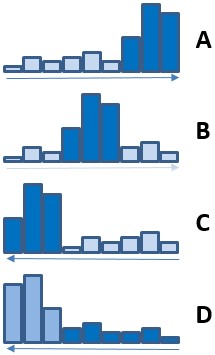
\includegraphics[scale=.7]{sections/images/consciousness_space_matter_antimatter.jpg}
	\floatfoot{Movements of matter and antimatter.}%\footnotemark}
	\end{figure}
	%\footnotetext{Fonte: note}

In example A, in Figure \ref{fig:consciousness_space_matter_antimatter}, the peak of the interval is to its right, which causes a higher velocity towards the population median. In example B, the peak is centered in the interval, however its samples are slightly more concentrated towards the population median, which causes a lower velocity in this direction and depending on the observer's point of view, this interval may appear to be going backwards. In example C, the peak of the interval is to its left, which causes a higher velocity as opposed to the population median and is more common in small intervals, however, the subintervals in dark blue (the peak), because they have more samples, tend to have their samples more easily towards the median and may move forward faster than the other subintervals, stabilizing the interval with the peak in the center or more to the right. Example D is similar to C, but the growth of the subintervals of this example are clearly in the opposite direction of the median of the population representing antimatter.

In Figure \ref{fig:consciousness_space_waves}, an example of the sample density of a population is shown, where pairs tending to the same probabilistic distribution are placed side by side and represented in histogram form. The formation of these pairs comes from wave entanglement.
	\begin{figure}[H]
	\caption{Entangled pairs represented in three spatial dimensions}
	\label{fig:consciousness_space_waves}
	\centering
	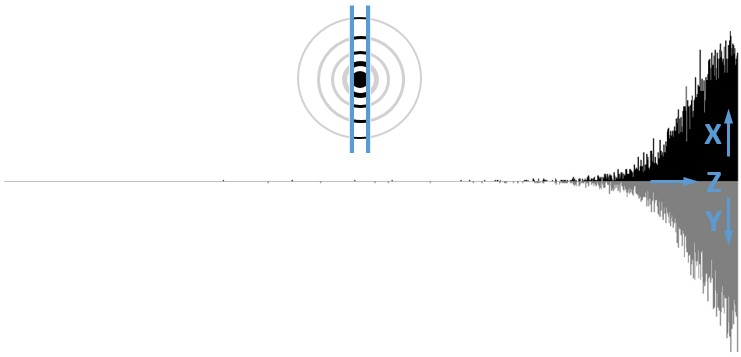
\includegraphics[scale=.7]{sections/images/consciousness_space_waves.jpg}
	\floatfoot{Example of entangled waves, represented in histogram form and obtained by the Logic\_WavePattern algorithm. \footnotemark}
	\end{figure}
	\footnotetext{The Logic\_WavePattern algorithm can be seen in Appendix \ref{app:algorithms}.}

By plotting the spatial dimensions of the graph of Figure \ref{fig:consciousness_space_waves} on a 3D distribution graph and distributing their endpoints (neglecting their volumes and possible internal points), something like a spiral is obtained (like eddies in water or air), even on very small data volumes (few logical moments), as in Figures \ref{fig:consciousness_space_3DScatter15000-10} and \ref{fig:consciousness_space_3DScatter_200000-2}. The points tend to move in a spiral shape approximately, as shown in the next subsection.
	\begin{figure}[H]
	\centering
		\begin{subfigure}[H]{0.47\linewidth}
		\centering
		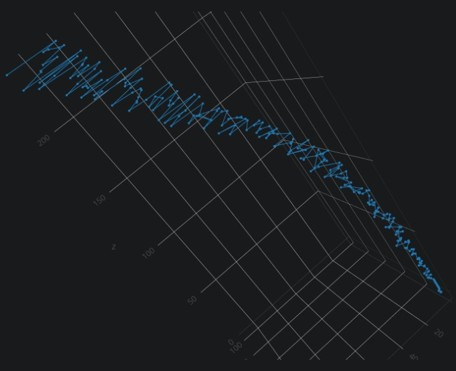
\includegraphics[width=1\linewidth]{sections/images/consciousness_space_3DScatter15000-10.jpg}
		\caption{15,000 samples or moments}
		\label{fig:consciousness_space_3DScatter15000-10}
		\end{subfigure}
	
		\begin{subfigure}[H]{0.47\linewidth}
		\centering
		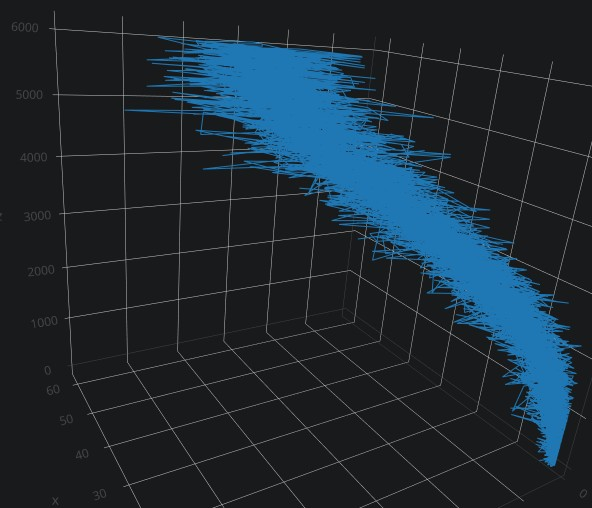
\includegraphics[width=1\linewidth]{sections/images/consciousness_space_3DScatter_200000-2.jpg}
		\caption{200,000 samples or moments}
		\label{fig:consciousness_space_3DScatter_200000-2}
		\end{subfigure}%
	\caption{3D scatter plots generated with points similar to Figure \ref{fig:consciousness_space_waves}}
	\floatfoot{The histogram on the wave pattern and the data for generating the 3D scatter plots can be obtained by running the Logic\_WavePattern algorithm. \protect\footnotemark}
	\end{figure}
	\footnotetext{The Logic\_WavePattern algorithm can be seen in Appendix \ref{app:algorithms} and the 3D scatter plots can be accessed at: \url{https://chart-studio.plot.ly/create/?fid=ren.stuchi:5&fid=ren.stuchi:4} e \url{https://chart-studio.plot.ly/create/?fid=ren.stuchi:7&fid=ren.stuchi:6}}

\subsubsection{Fundamental forces}
The gravitational force, the electromagnetic force and the nuclear force correspond to the so-called fundamental forces of nature. These fundamental forces are not forces as such, but probabilistic aspects of population distribution and wave entanglement.

\subsubsubsection{Gravitational force}
The gravitational force is not a force itself, but an aspect of the probability of distributing new samples towards the population median, according to the central limit theorem. This probabilistic sense makes waves have a probable path to follow within the population, that is, the peak of population samples or the peak of the largest wave in the population. In the same way, they also make the samples within an interval have a probable path to follow, the peak of samples of the interval or the peak of the wave. These sample peaks are usually the most easily observable part of the sample interval since they occupy a not so small area.

In Figure \ref{fig:consciousness_gravitational_force} it can be seen that the most easily observable part is slightly to the right at the peak of the wave. This wave tends to move up and to the right, in a diagonal direction to the peak of its upper interval. 
	\begin{figure}[H]
	\caption{Gravitational force}
	\label{fig:consciousness_gravitational_force}
	\centering
	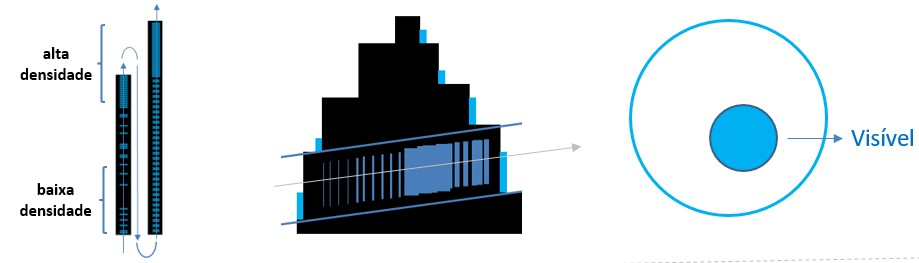
\includegraphics[scale=.7]{sections/images/consciousness_gravitational_force.jpg}
	\floatfoot{Gravitational aspect - the probabilistic direction of the distribution of new samples within an interval.}%\footnotemark}
	\end{figure}
	%\footnotetext{Fonte: note}

The area of an interval grows quadratically, since the jump caused by the entanglement of the waves and the probability distribution of the samples tends to maintain an equivalent growth in the pairs that form a wave. This aspect configures the inverse square law, where, in the case of gravity, the closer the objects, the greater the probabilistic chances of new samples of the smaller object heading towards the larger object (since the larger object tends to be the peak of wave - the probabilistic direction within the wave). Thus, for being within a smaller square area and, consequently, having less possibility of movement, it ends up increasing the chances of these objects approaching with a much smaller amount of logical moments. On the other hand, the more distant the objects, the larger the area, the greater the positioning possibilities and the more logical moments are needed for the approach, featuring less attraction. Probability can also drive away more rarefied objects that should be further away from the denser and more easily observable part of a wave, as in the case of helium gas, for example. The distribution of new samples in the rarefied intervals is slower than in the denser intervals (otherwise they would not be rarefied), so these dense particles receive more samples in a shorter amount of time, occupying the front of the less dense particles.

\subsubsubsection{Electromagnetic force}
The electromagnetic force is not a force in itself, but an aspect of the entanglement of waves that intensifies at intervals or wavelengths with low entropy and with the spatial approximation (reduction of differences in the X, Y and Z axes) of these intervals.

When intervals have low entropy, the total or partial overlapping of their areas facilitates the reordering of their entangled pairs, and an example of this can be the overlapping of an electron's area with the photonic clouds of other electrons or atoms. This reordering is an attempt to equalize these waves into a single low-entropy wave, which also makes it feasible to exchange many of these pairs for those of the non-entangled virtual cloud (virtual cloud of non-entangled samples, usually around the peak of the interval or subintervals, according to the subsection of Entanglement), which may result in the approximation of these waves due to this reordering.

The approximation of two magnets, for example, causes their virtual clouds to overlap and collide, causing movement and causing them to exchange entangled pairs among themselves and between the entangled intervals (entanglement of the same level), which establishes a synchronization of movements as the entanglements increase. This synchronization of movements will make these magnets approach each other in a specific and organized way due to the low entropy of their samples, always with their entanglements as close as possible, according to Figure \ref{fig:consciousness_electromaagnetic_force}, where the blue lines show where the exchange of pairs is more frequent of waves, that is, where there is a greater probability that the waves are similar. The entanglements synchronize the movements and tend to approximate the intervals as explained in the Space, Motion subsection.
	\begin{figure}[H]
	\caption{Electromagnetic force}
	\label{fig:consciousness_electromaagnetic_force}
	\centering
	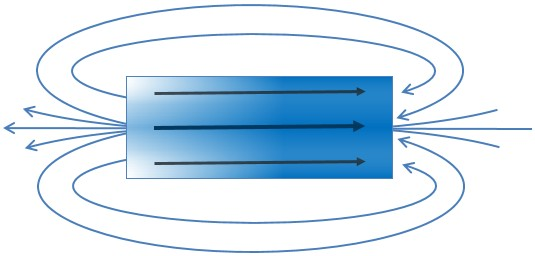
\includegraphics[scale=.9]{sections/images/consciousness_electromaagnetic_force.jpg}
	\floatfoot{Increased possibilities of wave entanglement due to probabilistic equalization in close and low entropy objects.}%\footnotemark}
	\end{figure}
	%\footnotetext{Fonte: note}

Figure \ref{fig:consciousness_electromaagnetic_force_entropy} shows an example of low entropy.
	\begin{figure}[H]
	\caption{Electromagnetic force - entropy}
	\label{fig:consciousness_electromaagnetic_force_entropy}
	\centering
	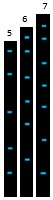
\includegraphics[scale=.9]{sections/images/consciousness_electromaagnetic_force_entropy.jpg}
	\floatfoot{Increased possibilities for wave entanglement due to low entropy.}%\footnotemark}
	\end{figure}
	%\footnotetext{Fonte: note}

The electromagnetic aspect is closely related to the low entropy of an interval and the possibility of entanglement of its pairs with surrounding pairs. The low entropy of an interval indicates that its samples are in some sort of order within it.

Probabilistically, the most similar wave pairs are found in the closest regions (blue lines in the figure \ref{fig:consciousness_electromaagnetic_force}). This occurs due to the growth of the number of samples towards the median of the population, however it is not a rule and the poles may reverse, that is, have more connections with the region of lower probability, even though most of the pairs that make up this region are increasing towards the median.

\subsubsubsection{Nuclear force}
The same probabilistic aspects that govern gravity and that can be seen in Figure \ref{fig:consciousness_gravitational_force} also govern the so-called nuclear forces. The difference is that in nuclear forces the intervals are smaller allowing a much larger amount of jumps and their waves are more discrepant, as shown in Figure \ref{fig:consciousness_space_subconsciousness_min}.

The strong and weak nuclear forces represent large concentrations of logic moments per population interval, a high density in a small interval. The large concentration of these samples is at the peak of the interval, which occupies a smaller and smaller subinterval within the wave (proportionately), due to the high concentration of samples in smaller and smaller intervals, as shown in Figure \ref{fig:total_comparison_chart_with_99_range}.

It is important to note in relation to the movements of electrons and atomic nuclei, as seen in the subsection of Orbits, that the atomic nucleus is moving as fast in space as all its higher waves. Star systems are at the same speed as their galaxies among others, due to the vigor of wave entanglement at all levels of entanglement, as per the subsection of Entanglement, making motion synchronous to a large extent. The nuclei, be they stellar, atomic or any other tend to be faster in space and pull their orbits, shown in the Orbits subsection. This synchronized and rapid movement in one direction of space does not cause repulsion.

The nucleus is a subinterval of the atomic interval (the wave peak). Electrons are also subintervals of the atomic interval, despite the high discrepancy between the atomic nucleus and its electrons. This discrepancy is common in small intervals such as the atomic one, as shown in Figure \ref{fig:consciousness_space_subconsciousness_min}, which tends to accentuate even more the discrepancy between the peak and the rest of the wave. However, in the subintervals of the peak or nucleus, this discrepancy is smaller because they are much denser than the electrons and are within the same probability distribution, approximately 99\% of the samples in the interval. Another factor that makes the discrepancy of the peak subintervals decrease even more is the abundance of these subintervals, so they tend to exchange subintervals with other atomic nuclei and fine-tune their sample distributions even more (movement and velocity, according to the corresponding ellipses in Figure \ref {fig:consciousness_space_dimensions}). Because they are close and with this greater correspondence, it increases the chances that they share more nested subintervals with each other, increasing the vigor between these subintervals of the same nucleus, which increases the correspondence of the movements between them, facilitating the approximation. In this way, it is easy to see that even in intervals with total vigor (where all the entangled subintervals are inside its upper interval) its subintervals are more or less separable as they are more or less entangled with each other (when the entanglement occurs in only one side of the pair because they are on the same level, according to the subsection of Entanglement).

Another important factor is that in smaller sample intervals, such as the nested subintervals of the atomic nucleus, it may be more common for them to behave like waves or more or less dense clouds, without a defined and visible peak, due to the tendency for their discrepancies to be larger as the subintervals decrease.

The penetration of these small and dense intervals by an excessive amount of logical moments (another similar interval), in a short period, causes the countless pairs of their subintervals to oscillate, potentiating the jumps. In this way the subintervals jump continuously, progressively and quickly until the probability distribution of the population normalizes the entire interval afterwards. Along with the jumps that will cause movements in large numbers of particles or intervals around them, there are a huge number of frictions at tremendous speeds caused by the collision of these small particles or clouds that cause great shock waves.

Since the subintervals of the atomic nucleus are very close and tuned in their motions and velocities, their entropies tend to be smaller. Therefore, when approaching two peaks with low entropies, the same effect tends to occur when trying to approach two magnets through the same pole, as explained in Figure \ref{fig:consciousness_electromaagnetic_force}.

\subsubsection{Spiral and orbit}
As the X, Y, and Z coordinates of the entangled pairs of a population tend to increase, their arrangement in a three-dimensional coordinate system will follow a diagonal reference between these three axes, as shown in Figure \ref{fig:consciousness_space_spiral_reference_line}. The observed spiral pattern does not invalidate other possible movements in space. Often, it is not possible to immediately observe the spiral pattern in the movements of an interval (subinterval), yet this pattern underlies many of these movements.  Taking human movements, for example, there are predominant cycles of going and coming home, going to and from work, waking up and sleeping, that is, habits are similar to movements in cycles (spiral movements).
	\begin{figure}[H]
	\caption{Three-dimensional coordinate system}
	\label{fig:consciousness_space_spiral_reference_line}
	\centering
	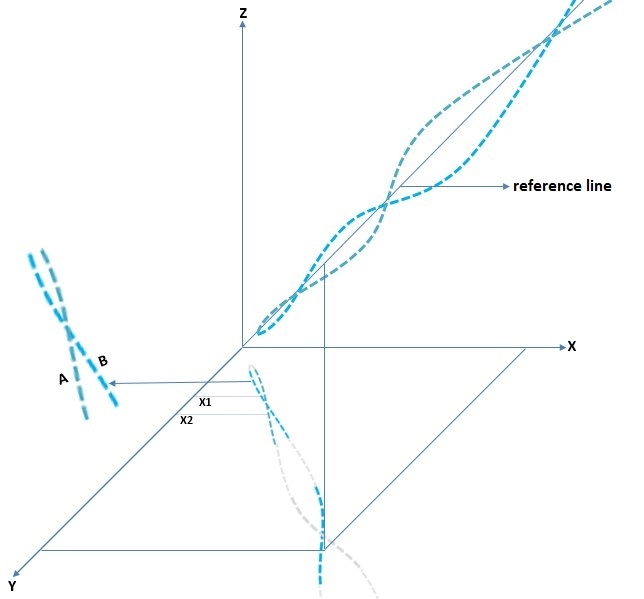
\includegraphics[scale=.7]{sections/images/consciousness_space_spiral_reference_line.jpg}
	\floatfoot{Probabilistic reference line for distribution of a population in a three-dimensional plane.}%\footnotemark}
	\end{figure}
	%\footnotetext{Fonte: note}}

In Figure \ref{fig:consciousness_space_spiral_reference_line} points X1 and X2 can also be observed. These points were mirrored in X and Y coordinates to facilitate the observation that even at the bottom of the spiral the interval continues to add samples, albeit in smaller amounts than when going up to the top of the spiral. The dashed lines show the most probable paths to the A and B intervals. Thus, when a part of the interval is at its maximum midpoint (X and/or Y axes) the probabilistic tendency is that it receives fewer samples than the part of the interval that is at its minimum midpoint. This spiral effect is more noticeable the larger an interval and its quantity of samples, as the more probable and stable these paths will be.

The continuous motion in a rarefied environment also helps in the formation and maintenance of the spirals. As the samples are added to the subintervals their velocities tend to increase towards the reference line, and because this addition is not uniform (varying between peaks and valleys) and the motion is approximately continuous the subintervals can drift or slide from one side of the reference line to the other.

Each interval or subinterval (wavelength) has its own reference line. Just as within a meter there are centimeters, millimeters, etc., within an interval and subinterval there can be numerous other subintervals.
	\begin{figure}[H]
	\caption{Intervals and reference lines}
	\label{fig:consciousness_space_spiral_underlines}
	\centering
	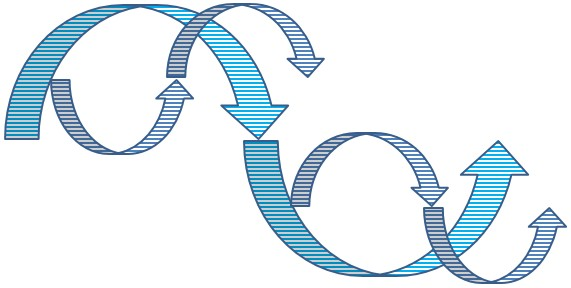
\includegraphics[scale=.5]{sections/images/consciousness_space_spiral_underlines.jpg}
	\floatfoot{Spirals at different intervals and their reference lines.}%\footnotemark}
	\end{figure}
	%\footnotetext{Fonte: note}}

\subsubsubsection{Orbits}
Orbit can be defined in this study as the concept of the spirals plus the orientation of a probabilistic peak (gravity) instead of the reference line of the spirals, only.

Systems that orbit as described earlier (in spiral - oriented by the reference line) are systems or intervals in which their peak is subdivided into subintervals and do not form a center of gravity, that is, all subintervals of the peak are not concentrated in one point of the system, thus orbiting the reference line of the interval. Probably galaxy clusters and superclusters are examples of this orbit. The spiral orbit (oriented by the reference line) is not restricted to large systems, this orbit is a feature that can happen in any size of interval.

Another type of orbit is defined when the subintervals that orbit the peak of the wave (which represents approximately 99.9\% of the samples in the interval) decrease their orbit speed as they move away from the peak. In Figure \ref{fig:consciousness_elliptical_orbit_system} the columns of the histogram in blue represent the peak of the wave. This decrease in velocity occurs gradually as these gray intervals move away from the peak of the wave, thus receiving a smaller amount of samples decreasing their acceleration. The solar system is possibly an example of this type of orbit. Atomic orbits may also resemble this type of orbit due to the differences in energies between the layers structured by the jumps.  
	\begin{figure}[H]
	\caption{Orbits of the subintervals outside the wave peak}
	\label{fig:consciousness_elliptical_orbit_system}
	\centering
	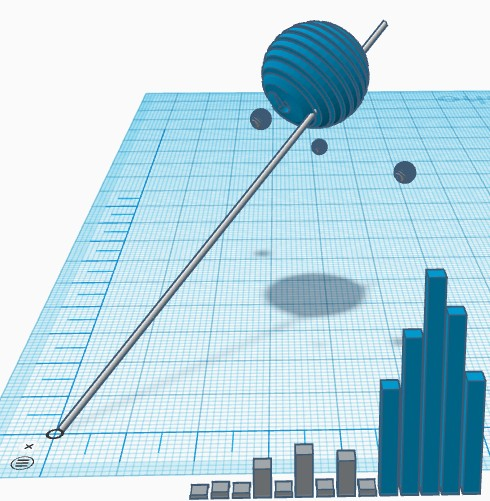
\includegraphics[scale=.7]{sections/images/consciousness_elliptical_orbit_system.jpg}
	\floatfoot{The subintervals decrease in speed as they move away from the peak of the wave.}%footnotemark}
	\end{figure}
	%\footnotetext{Fonte: note}

Yet another type of orbit is defined when the subintervals that orbit the peak of the wave maintain a constant average velocity regardless of the distance from the peak. This occurs because these subintervals are also part of the wave peak in blue, as shown in Figure \ref{fig:consciousness_circular_orbit_system}. Thus, because these subintervals remain in orbit within the 99.9\% subinterval of the wave, their velocities do not decrease. This 99.9\% of the wave is most easily visible part, therefore, the observed part of the galaxies, probably. Perhaps this feature is also responsible for the rings of planets.
	\begin{figure}[H]
	\caption{Orbits of the subintervals inside the wave peak}
	\label{fig:consciousness_circular_orbit_system}
	\centering
	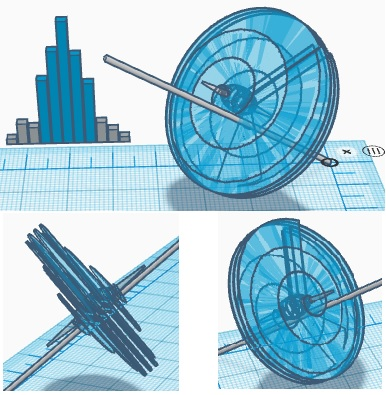
\includegraphics[scale=.9]{sections/images/consciousness_circular_orbit_system.jpg}
	\floatfoot{The subintervals maintain their speed as they move away from the peak of the wave.}%\footnotemark}
	\end{figure}
	%\footnotetext{Fonte: note}

For the distance of the subintervals in orbit, gravity exerts more of an orientation than an attraction. But since the motion is practically continuous in rarefied environments and this orientation is permanent, the orbits are formed and maintained by the increasing speed of these subintervals, which tends to pull them apart.

As stated in the subsection of space, a new sample in a subinterval moves it and its upper intervals. Also new samples in the upper interval move the lower intervals, as they are fractions of the same wave. In this way, a lower wave will remain in the upper wave when its velocity is less than the peak velocity of the upper wave and its path is not opposite to the upper wave's path. The movement of the upper wave drags its subintervals, which with lower probabilistic speeds will continue to move within its upper wave, because even with lower speeds they are dragged by the movement of the upper wave, which is also composed of the movement of its subintervals.

Doubling the amount of samples in an interval will not definitely double the speed of an interval, as it have twice as many samples to move, leaving the velocity unchanged. However, probabilistically, the greater the number of samples of a wave, the more these samples will be towards the population median and the less relevant the contrary samples become, which makes the probabilistic speed of wave peaks higher than the speed of their subintervals. This is not a rule and a subinterval may have a velocity greater than the peak of its upper wave or its movement may be contrary to the movement of the peak of the upper wave, causing it to naturally exit the gravitation of its upper wave (and this occurs more easily with very small and fast intervals favored by its movement in a rarefied environment due to its size).

\subsubsubsection{Dark matter and dark energy}
Major subintervals move apart, even though they maintain a common path. This occurs due to the probabilistic aspect of expanding the subintervals of a superior interval with the addition of new samples, as evidenced in the histogram columns of Figure \ref{fig:consciousness_circular_orbit_system}. The expansion happens in all the subintervals of an interval, however it is more expressive at the peak of larger waves due to the greater amount of new samples. The subintervals naturally move apart due to increasing speeds, as they receive more samples at their peak, and the greater this imbalance or disproportion of samples within an interval, the faster it will be, according to the Space subsection. The more distant subintervals tend to be faster, as they are normally part of the peak subintervals, in blue in Figure \ref{fig:consciousness_circular_orbit_system}, which receive more samples.

Spirals can occur without the need for a concentrated wave peak, but when there is such a concentration in the wave peak, orbits can occur within or outside of 99.9\% of peak samples, resulting in orbits that maintain their average velocity constant when away from the peak (within 99.9\%) or orbits that decrease their velocities when away from the peak (out of 99.9\%).

Therefore, dark matter and dark energy are neither matter nor energy, but probabilistic aspects of the distribution of samples in a population that resembles the normal distribution.

\subsubsection{Antimatter}
When an interval tends to concentrate its samples toward the median, which is the probable direction according to the central limit theorem, it is called matter. Antimatter is the opposite, when an interval tends to concentrate its samples in the direction opposite to the median. 

The simplest way to visualize the probabilistic direction of samples of any wavelength is to look at the \textbf{probabilistic reference line}, as shown in Figure \ref{fig:consciousness_space_spiral_reference_line}. The greater the amount of sample in an interval, the greater will be its probabilistic tendency towards the population median.

In the Figure \ref{fig:consciousness_concentration_of_opposite_samples} two identical intervals are shown with their samples at opposite concentrations.
	\begin{figure}[H]
	\caption{Identical interval with its opposite sample concentrations}
	\label{fig:consciousness_concentration_of_opposite_samples}
	\centering
	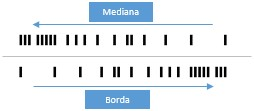
\includegraphics[scale=1.2]{sections/images/consciousness_concentration_of_opposite_samples.jpg}
	\floatfoot{Identical interval distributed in opposite ways.}%\footnotemark}
	\end{figure}
	%\footnotetext{Fonte: note}

Merging or summing the opposite intervals in Figure \ref{fig:consciousness_concentration_of_opposite_samples} would make them a symmetric interval, that is, it would not be in any direction.
The figure \ref{fig:consciousness_concentration_of_opposite_samples_within_range} shows one population with its samples concentrated toward the median and another with its samples concentrated toward the interval boundaries.
	\begin{figure}[H]
	\caption{Populations with their opposite sample concentrations}
	\label{fig:consciousness_concentration_of_opposite_samples_within_range}
	\centering
	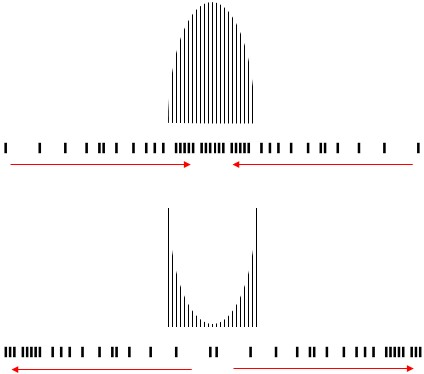
\includegraphics[scale=.7]{sections/images/consciousness_concentration_of_opposite_samples_within_range.jpg}
	\floatfoot{Populations distributed in opposite directions.}%\footnotemark}
	\end{figure}
	%\footnotetext{Fonte: note}

\subsubsection{Black Hole}
The area of an interval grows as new samples are added into the population, as Figure \ref{fig:consciousness_space_volume_amplitude}, and with the addition of other already entangled intervals, as shown by the upper right subinterval in Figure \ref{fig:consciousness_interval_contraction}. However, intervals that receive a large amount of samples within the population tend to form more and more subintervals at different levels, which contracts the occupied area of these intervals (because of the wave entanglement from the smaller subintervals sustaining these approximately quadratic areas) as shown by the purple and blue subintervals in Figure \ref{fig:consciousness_interval_contraction}. So this relationship of the size of the interval with its amount of samples and their subintervals is the aspect that can help describe the so-called black holes, where the peak of the wave will occupy a smaller and smaller proportional subinterval within the interval of the wave, even with an increasing concentration of samples. These peaks are often found from the middle to the front of an interval or system (the core or peak of the system).
	\begin{figure}[H]
	\caption{Interval contraction}
	\label{fig:consciousness_interval_contraction}
	\centering
	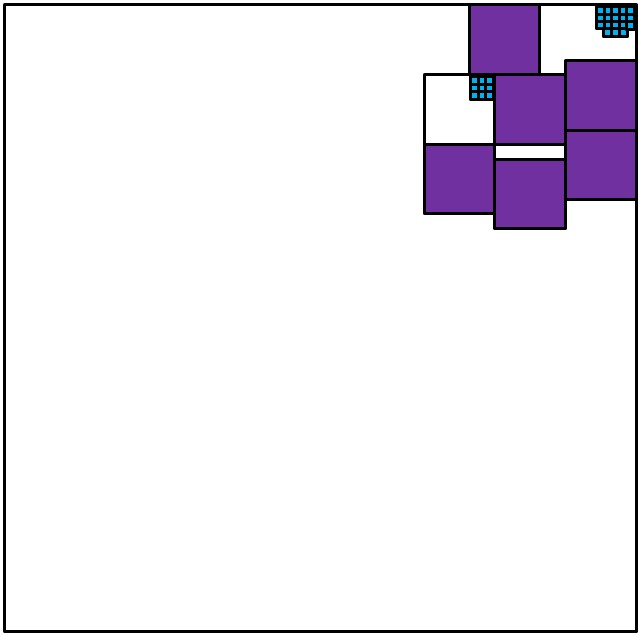
\includegraphics[scale=.5]{sections/images/consciousness_interval_contraction.jpg}
	\floatfoot{Relationship of interval size and its possible contraction as new subintervals appear.}%\footnotemark}
	\end{figure}
	%\footnotetext{Fonte: note}
	
\subsubsection{Observer and life}
The wave intervals (wavelengths) that a subconsciousness (sublogic) is able to observe depend on the wavelengths of which the subconscious itself is composed. Among all the possibilities of intervals or wavelengths allowed by a population, the observer is in one of them. 

The ability to compare or distinguish the order of changes in a sequence of samples is the logical ability of an observer, the observer of time (past and present).The speed of this observation is given by the range that the observer is able to compare, that is, how quickly the observer is able to distinguish small changes (few samples - few logical moments) will make it realize that larger changes take longer (many samples - many logical moments).

The logical ability to make probabilistic prospections, within the logical limitations of the observer and based on the probability of distribution of the observed interval or subinterval, is the essence of thinking and, therefore, of life. These prospections are based on the probability of distribution of each interval (in the direction of the interval) and, therefore, are related to pattern detection and future probabilistic possibilities.

The ability to compare or distinguish logical waves (subsets or subconscious) is the ability that defines the subject [I - me]. The reasonableness of this definition depends on the proportionality of this ability to compare.

Typically, the most notable life forms are multiplied by being on the probabilistic average of the interval between their peaks and valleys, however different they may be. Something very discrepant or different from the average pattern of the interval tends not to multiply and remain.

Life \underline{IS NOT}, like any other logic. And its meaning lies in what logic is in its essence. Logic in its probabilistic essence is the order that emerges from the chaos of infinite possibilities, it is what physics calls gravity and the Bible calls Love when it says that God is Love. Therefore, the meaning of life is to be different, which in contrast to a straight line (representing nullity, indifference or non-existence) becomes discrepant with its peaks (waves), peaks that entangle and share their subintervals with the others of their waves, making their movements and their subintervals more harmonious and synchronized, which in some scales are called orbits in others love, when the human being orbits that which he loves, whatever it is. This is the meaning of life and of the whole universe, and not only this, besides giving meaning is what makes them possible. The human being can perhaps be considered the peak of the wave of the subsystems considered to be alive on earth, having the capacity to dominate and care for the others.

The free will is in the randomness of the new samples, despite the probabilistic sense of these samples toward the median of the population. And that is the only way to be exceptionally free from the cause and effect or action and reaction that predominate in all movement. So it can be argued that anything a person has done is the fault of the universe, or moreover, the fault of logic that \underline{IS NOT}, rigorously what the universe and men are. The relevant fact is that all possibilities are valid and perhaps this is the greatest justice of all. Considering something or someone guilty or anything else is part of these possibilities, so the essence of the world is in the difference and every different movement tends to have different reactions.

\subsubsubsection{Senses}
The cognitive part of a wave is not observed directly, but rather the outside - the consciousness, the whole or more commonly a part of that whole. This observation may include the rest of the wave that the cognitive part is part of, which is also external to the cognitive part, and so the cognitive part may be a nested subinterval of another. The cognitive part of the human subconscious is probably where the largest wave peak of the human subset is found. This is where the greatest intensity of change is observed. This great intensity of change is largely characterized by human thinking (observation and probabilistic prospecting of an interval) that tends toward infinity, as well as the essence of logic, the [NOT BEING].In other words, the cognitive part is the part that is closest to logic in its essence and also to its totality (consciousness).

The taking of samples by human beings, through the senses, modifies them and these ripples act as adjustments or configurations. Each sense observes the sample population independently, as distinct frequency channels. Thus, eyesight can be seeing objects very far away and ears hearing sounds that are very close. The senses are limited by the waves that constitute the observer and their maximum observation capacity is limited in the maximum depth of the nested intervals observed.

An important feature of the process of observing small intervals is that they can be observed with particles or waves. In particle observation, the observer follows an interval represented by an entangled pair, observing its consistent shape and movement in space. In the particle effect, the consistency of the shape and its movements are established by the entangled pair, since the jump occurs on one side of the pair at a time, guaranteeing stability in the changes. In the interval observed as a wave, the observer follows one of the parts that make up the entangled pair, observing its movements and jumps, since the jumps are frequent in small intervals.

It may not be possible to observe the wave effect without entangling its pair. The high frequency of this interval causes it to rapidly transit in an area around it, which may make it easier for it to reach a specific point in space, such as the human eye, that collapses its particle effect. This collapse can occur in a wider location (such as a wall or screen), and observe its wave effect with the collapse of many samples.
